

\section{Questão 5}

\subsubsection{Através da opção tcpdump verifique e compare como flui o tráfego nas diversas interfaces do dispositivo de interligação no departamento A (LAN partilhada) e no departamento B (LAN comutada) quando se gera tráfego intra-departamento (por exemplo, fazendo ping IPaddr da Bela para Monstro, da Jasmine para o Alladin, etc.) Que conclui?}

    \begin{figure}[H]
    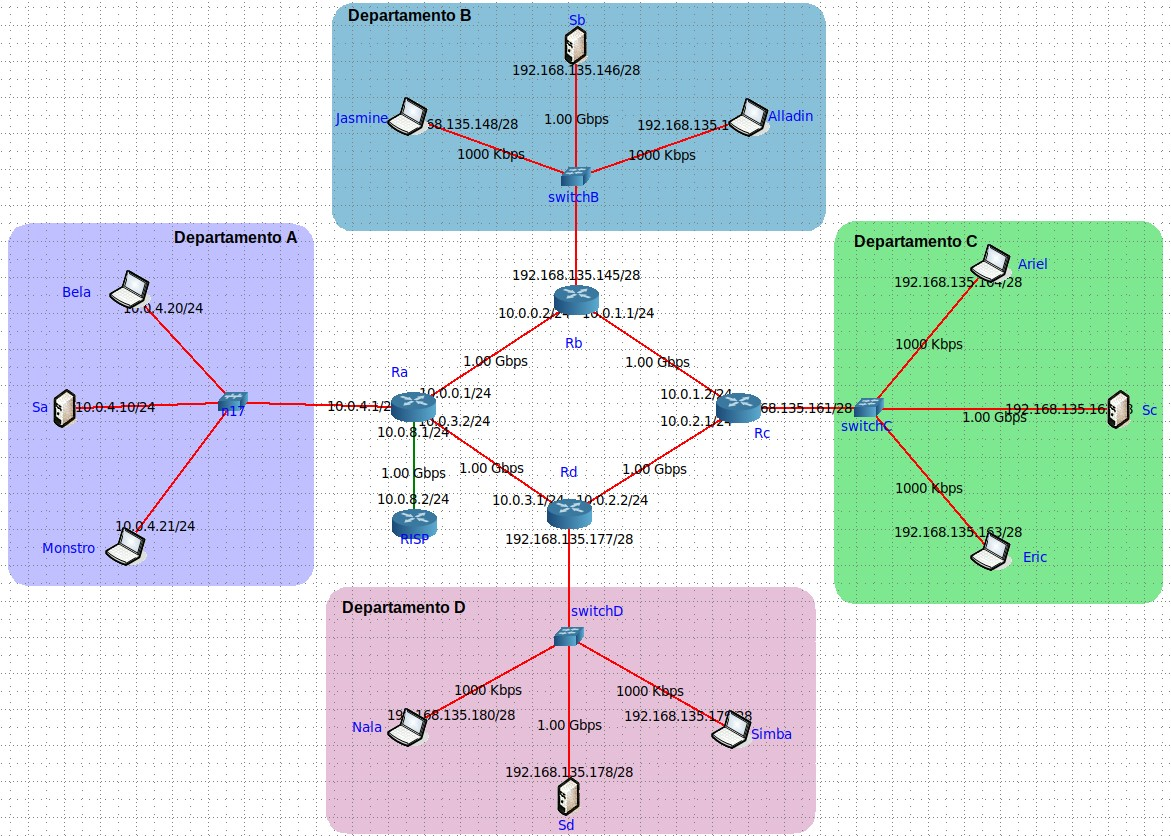
\includegraphics[width=\linewidth]{prints/Questao5/topologia.jpg}
    \caption{Topologia com o \textit{hub} adicionado.} 
    \label{questao5-topologia}
    \end{figure}
    

    \par Como podemos ver pela Figura \ref{questao5-topologia}, os endereços IP dos dispositivos Bela, Monstro e servidor Sa foram alterados em consequência da inserção do \textit{hub} e remoção do \textit{switch}. No entanto, o grupo optou por não voltar a alterar os endereços para os obtidos com o exercício de \textit{subnetting} do trabalho prático anterior, uma vez que não não iria alterar o comportamento esperado neste exercício em particular. Os testes foram realizados da seguinte forma: executou-se um \textit{ping} de um \textit{host} A para outro \textit{host} B e executou-se o comando \textit{tcpdump} num \textit{host} C não envolvido na comunicação do \textit{ping}. Assim, no \textbf{departamento A} executamos o comando \textit{ping} do \textit{host} Monstro para Bela e o comando \textit{tcpdump} no servidor Sa. No caso do \textbf{departamento B}, executamos o comando \textit{ping} do \textit{host} Alladin para Jasmine e o comando \textit{tcpdump} no servidor Sb. Por fim, obtivemos os seguintes resultados com os vários comandos:
            
            
    \begin{minipage}{0.5\linewidth}
        \centering
            \begin{figure}[H]
            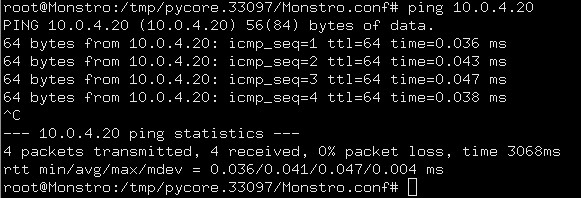
\includegraphics[width=\linewidth]{prints/Questao5/A-Monstro-Bela.jpg}
            \caption{Ping do \textit{host} Monstro para Bela.} \label{questao5-ping-A}
            \end{figure}
    \end{minipage}
    \begin{minipage}{0.5\linewidth}
        \centering
            \begin{figure}[H]
            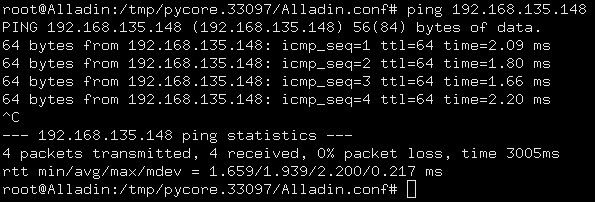
\includegraphics[width=\linewidth]{prints/Questao5/B-Alladin-Jasmine.jpg}
            \caption{Ping do \textit{host} Alladin para Jasmine.} \label{questao5-ping-B}
            \end{figure}
    \end{minipage}

    \paragraph{}
    \paragraph{}
    \begin{figure}[H]
    \centering
    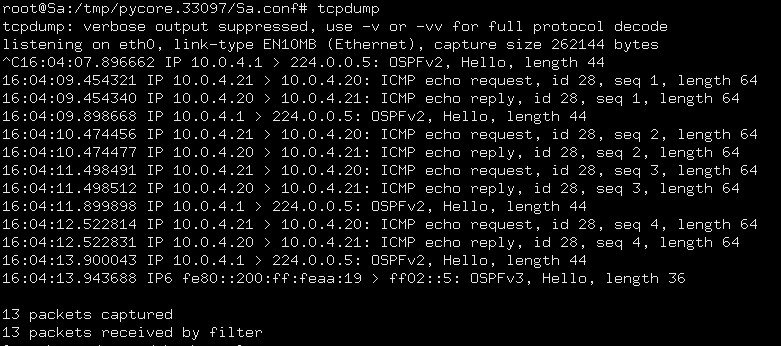
\includegraphics[width=400pt]{prints/Questao5/A-Sa.jpg}
    \caption{Comando \textit{tcpdump} no servidor Sa (LAN partilhada).} \label{questao5-tcpdump-A}
    \end{figure}
    
    \begin{figure}[H]
    \centering
    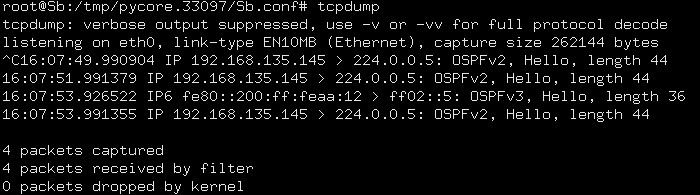
\includegraphics[width=400pt]{prints/Questao5/B-Sb.jpg}
    \caption{Comando \textit{tcpdump} no servidor Sb (LAN comutada).} \label{questao5-tcpdump-B}
    \end{figure}
    
    
    
    \par Existem várias diferenças entre \textit{hubs} e \textit{switches}, sendo a mais distinta a camada protocolar onde operam, isto é, o \textit{hub} opera ao nível físico enquanto que os \textit{switches} operam na camada de ligação lógica.
    Para além disto, os \textit{\textbf{hubs}} são dispositivos que repetem o sinal que chega através de uma porta de entrada para todas as outras portas, isto é, difundem o sinal por todas as interfaces que possuem.
    No que toca aos \textit{\textbf{switches}}, estes, com a ajuda de uma tabela de \textit{switching} (comutação), comutam as tramas para a interface de saída apropriada. No entanto, caso se depare com uma trama que não tem um endereço que conste na tabela, este difunde a trama por todas as suas interfaces, obtendo, neste caso em específico, um comportamento semelhante ao \textit{hub}.

    \par Assim, e tendo estas distinções em mente, conseguimos de imediato notar diferenças no resultado do comando \textit{tcpdump} nas duas situações. Na \textbf{LAN partilhada}, o terceiro \textit{host} não envolvido diretamente na comunicação também recebeu os pacotes, provando assim a particularidade dos \textit{hubs} no que toca à difusão das comunicações por todas as portas dos mesmos.
    No caso da \textbf{LAN comutada}, denotamos que o resultado da captura é vazio no que toca a pacotes relacionados com a comunicação derivada do comando \textit{ping}, provando assim a diferença de comportamento do \textit{switch} com o \textit{hub}, pois o tráfego é comutado para as interfaces devidas, não sendo difundido pela rede.




%\newpage
\subsubsection{Construa manualmente a tabela de comutação do switch do Departamento B, atribuindo números de porta à sua escolha.}

    \paragraph{}
    \par Para obtermos os endereços MAC dos vários sistemas diretamente ligados ao \textit{switch}, executamos o comando \textit{\textbf{ifconfig -a}}. Assim, obtivemos os seguintes endereços, notando que no \textit{router} o endereço da interface \textit{eth2} corresponde à interface de ligação ao \textit{switch}.

    \begin{minipage}{0.5\linewidth}
        \centering
            \begin{figure}[H]
            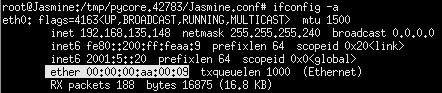
\includegraphics[width=\linewidth]{prints/Questao5/Jasmine.jpg}
            \caption{Endereço MAC Jasmine.} \label{questao5-MAC-Jasmine}
            \end{figure}
    \end{minipage}
    \begin{minipage}{0.5\linewidth}
        \centering
            \begin{figure}[H]
            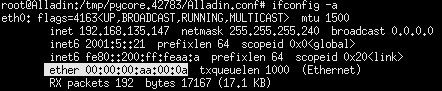
\includegraphics[width=\linewidth]{prints/Questao5/Alladin.jpg}
            \caption{Endereço MAC Alladin.} \label{questao5-MAC-Alladin}
            \end{figure}
    \end{minipage}
    
    \begin{minipage}{0.5\linewidth}
        \centering
            \begin{figure}[H]
            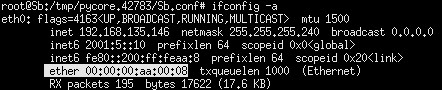
\includegraphics[width=\linewidth]{prints/Questao5/Servidor.jpg}
            \caption{Endereço MAC Servidor.} \label{questao5-MAC-Servidor}
            \end{figure}
    \end{minipage}
    \begin{minipage}{0.5\linewidth}
        \centering
            \begin{figure}[H]
            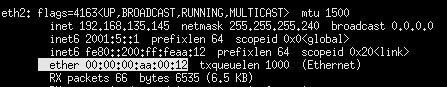
\includegraphics[width=\linewidth]{prints/Questao5/Router.jpg}
            \caption{Endereço MAC Alladin.} \label{questao5-MAC-Router}
            \end{figure}
    \end{minipage}
    
    \paragraph{}
    \par Após obtermos os endereços MAC, desenvolvemos um esboço da topologia da subrede do Departamento B (incluindo o \textit{router}) para assim termos uma visão simplificada dos sistemas integrantes. Como tal, obtivemos a seguinte tabela de comutação:
    
    \begin{figure}[H]
    \centering
    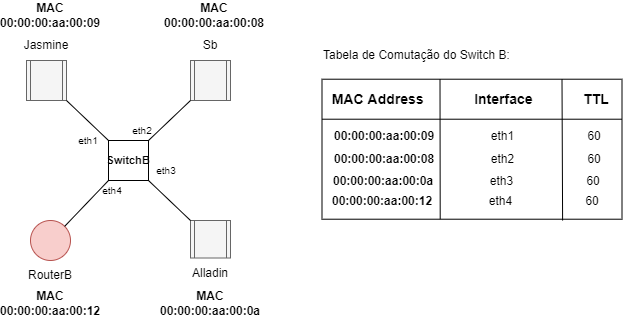
\includegraphics[width=450pt]{prints/Questao5/switch.png}
    \label{questao5-switchTable}
    \end{figure}